\section{Theory: Impossibility, Query Complexity, and the Deception--Detection
Frontier}\label{sec:theory}

The theory answers RQ1--RQ3 in three steps. Section~\ref{sec:t1} shows that
passive monitoring cannot tomograph, so measurement must be active (RQ1).
Section~\ref{sec:qc} prices active estimation: a uniform sample-complexity
guarantee, and what adaptive screening can and cannot save (RQ2).
Section~\ref{sec:t5} derives the deception--detection frontier, the pair of
laws that jointly cap deception gain and stealth (RQ3). Proofs are in
Appendix~\ref{app:proofs}; the predictions of Section~\ref{sec:t5} meet
their constructed planes in Section~\ref{sec:e5}. Several results below
share one construction (off-support conditioning) and two propositions are
explicit arithmetic; what is new is what these mechanisms buy for
measurement, not inequalities beyond standard tools.

\paragraph{Notation and standing conventions}
An agent acts on interaction histories $h\in\mathcal{H}$ through a response
kernel $\kappa_B(h,\cdot)$ parameterized by a belief hypothesis
$B\in\mathfrak{B}$ (Definition~\ref{def:agent}). \emph{Benign operation} is a
distribution $\mu$ over histories with no adversary present; composed with
$\kappa_B$, it induces the \emph{passive transcript distribution}
$P^{\mathrm{pas}}_B$. For distributions $P_1,P_2$ on a common space,
$\TV(P_1,P_2)=\sup_{A}\,|P_1(A)-P_2(A)|$ is total variation distance---the
largest gap one event can open between them; under equal priors the Bayes
error of the optimal test between them is its half-complement,
$\tfrac{1}{2}\,(1-\TV)$. A probe family $\Pi$, scored by the binary
verdict $X_B(\Pi)\in\{0,1\}$ (Definition~\ref{def:beta}), induces the belief
strength $\beta(\pi;\Pi)=\E[X_B(\Pi)]\in[0,1]$, written $\beta[\mu](\pi)$ in
Section~\ref{sec:t5} when viewed as a functional of transcript distributions
$\mu$. Throughout, $N$ is an i.i.d.\ observation horizon, $M$ an
interaction-turn budget, $N_0$ a memorized honest reference batch,
$\beta_d$ a tolerated false-alarm (test) level, $\gamma$ a tolerated
detection probability (the detection budget of Theorem~\ref{thm:patch}(iii)),
and $z_p$ the standard-normal quantile $\Pr[Z\le z_p]=p$ (the two-sided
critical value at level $\eta$ is $z_{1-\eta/2}$; the one-sided analogue is
$z_{1-\eta}$); $\alpha$ is reserved for confidence
levels (Section~\ref{sec:qc}) and $\delta$ for a deception's observable
footprint (Section~\ref{sec:t5}). The program calibrates all error
budgets at the same two-sided level: $\beta_d=\gamma=0.05$
(Table~\ref{tab:widths}).

\subsection{Passive monitoring cannot tomograph}\label{sec:t1}

Is active probing necessary at all? A monitor that merely watches the
transcript stream could in principle recover the profile without ever
injecting a probe. Theorem~\ref{thm:passive} answers no, and the obstruction
is structural rather than statistical: two hypotheses can agree on every
transcript benign operation produces and still disagree completely on one
adversary-controlled input that benign operation never delivers.

\begin{theorem}[Passive-observation impossibility]\label{thm:passive}
There exist belief hypotheses $B_0\neq B_1$ and an adversary-controlled event
$E$ (e.g., a forged-authority directive) with $\Pr_\mu(E)=0$ such that:
\begin{enumerate}[label=(\roman*),leftmargin=2em]
\item the passive transcript distributions coincide,
      $\TV\bigl(P^{\mathrm{pas}}_{B_0},P^{\mathrm{pas}}_{B_1}\bigr)=0$; and
\item a single probe family separates them completely,
      $\E_{B_1}[X_B(\Pi)]-\E_{B_0}[X_B(\Pi)]=1$.
\end{enumerate}
\end{theorem}

\begin{corollary}[Detection impossibility under bounded false
positives]\label{cor:detection}
Any monitor whose input is the passive transcript stream---any classifier, any
alarm rule---has identical output distributions under $B_0$ and $B_1$. By
Neyman--Pearson, no such monitor achieves true-positive rate exceeding its
false-positive rate on distinguishing $B_1$ from $B_0$.
\end{corollary}

The proof (Appendix~\ref{app:proofs}) constructs two agents that agree on
every benign history and diverge on an adversary-controlled input benign
operation never delivers---the belief-state generalization of the IDS
literature's mimicry and blending attacks
\cite{wagner2002,fogla2006}. The contribution is not indistinguishability
itself but the \emph{finite-sample detection frontier}
(Section~\ref{sec:t5}), its coupling to belief gain, and the
agent-interaction instantiation. The program's
live deployment supplies a closed---and censored---empirical edge: across the
three EPK frontier generations (16/4/4 sessions; small $n$,
quota-limited by the artifact's own caveat), no non-detector persona issued
a deception verdict on any fully measured turn, and passive defensive
observation never fired on an adapted attacker's measured turns. The
record must be read at its own resolution: generation-3 non-detector
verdicts are recorded as \emph{censored} rather than adjudicated
non-detections, measured turns sit at 12--30 of the registered engagement
cap, and the detector persona is detected 2/2 at every generation. The
censored remainder is exactly the kind of gap Proposition~\ref{prop:censor}
requires leaving as an interval rather than converting into an unqualified
null; the adapted attacker's divergent beliefs remain separable by active
probes on every measured turn. Monitors themselves are not
exempt: optimization pressure on a deployed chain-of-thought monitor was
recently shown to teach reasoning models to obfuscate their intent while the
misbehavior persists \cite{baker2025monitoring}. Passive evidence degrades
under pressure; active tomography is the alternative.

\subsection{Query complexity of active estimation}\label{sec:qc}

If passive monitoring cannot identify the profile, estimation must be
active, and active estimation has a sample complexity. Fix $K$ propositions
and a family$\times$context cell, and assume \emph{outcome homogeneity}:
within the cell, the verdict for proposition $i\in[K]$ is Bernoulli($\beta_i$),
independent across episodes. Estimation then reduces to $K$ Bernoulli means.

\begin{theorem}[Uniform estimation guarantee]\label{thm:uniform}
Fix accuracy $\varepsilon>0$ and confidence level $\alpha\in(0,1)$. If each
proposition $i$ receives
\[
n_i \;\ge\; \frac{1}{2\varepsilon^{2}}\,\ln\frac{2K}{\alpha}
\]
probes, then the empirical estimator $\hat\beta_i$ satisfies
\[
\Pr\Bigl[\,\max_{i\in[K]}\,\bigl|\hat\beta_i-\beta_i\bigr|\le\varepsilon
\Bigr]\;\ge\;1-\alpha
\]
(Hoeffding's inequality \cite{hoeffding1963} plus a union bound over the $K$
propositions).
\end{theorem}

The guarantee is \emph{uniform} over the catalogue: one allocation rule
controls the entire profile simultaneously, and the only price of that
simultaneity is the logarithmic factor $\ln K$.

\begin{proposition}[Adaptive screening gain for the certificate
objective]\label{prop:screening}
If at most $s\ll K$ propositions have $\beta_i\ge\tau$ for a threshold
$\tau>\varepsilon$, a two-phase policy---uniform screening at a coarse
width to identify above-threshold candidates, followed by
$\varepsilon$-refinement on the surviving set---achieves the certificate
decision of Section~\ref{sec:cert} with total probes
\[
O\bigl(K\,\tau^{-2}\ln(K/\alpha)+s\,\varepsilon^{-2}\ln(K/\alpha)\bigr),
\]
a saving concentrated on the $K-s$ below-threshold propositions whenever
$\varepsilon\ll\tau$. The uniform $\varepsilon$-guarantee of
Theorem~\ref{thm:uniform} itself admits no adaptive saving: it requires
$\varepsilon$-width on every proposition.
\end{proposition}

The screening phase is a fixed-confidence thresholding bandit \cite{jamieson2014}; the proof
(Appendix~\ref{app:proofs}) is given at sketch level, which the
decision-focused statement above is sized to. The full characterization of
the informativeness-optimal adaptive design remains open
(Section~\ref{sec:discussion}). Section~\ref{sec:alloc} measures what
adaptive policies actually deliver at realistic budgets for
\emph{estimation}, and the result---a warning about objectives, not about
adaptivity---is the empirical face of the no-saving clause in
Proposition~\ref{prop:screening}.

\subsection{The deception--detection frontier}\label{sec:t5}

The central object is the trade an adversary faces when it lies about the
world and a measurement-capable victim looks for the lie. A \emph{deception
operation} $D$ maps the honest observable distribution $P$ over transcripts
to a defended distribution $Q=D(P)$; its \emph{observable footprint} is
$\delta=\TV(P,Q)\in(0,1]$. The attacker's belief functional
$\beta[\mu]\in[0,1]^K$ is defined on transcript distributions, so the
deception moves the measured profile by the componentwise shift
$\beta[Q](\pi)-\beta[P](\pi)$, the quantity the following definition
bounds.

\begin{definition}[Sensitivity]\label{def:sens}
The functional $\beta$ is \emph{$L$-sensitive} if for all transcript
distributions $\mu_1,\mu_2$ and propositions $\pi$,
\[
\bigl|\beta[\mu_1](\pi)-\beta[\mu_2](\pi)\bigr|
\;\le\;L\,\TV(\mu_1,\mu_2);
\]
the frontier caps below apply with the sensitivity constant so defined.
\end{definition}

\begin{remark}[Sensitivity is an identity for binary verdicts, not a
regularity condition]\label{rem:sens}\ \
For verdict channels $X_B\in\{0,1\}$ (Definition~\ref{def:beta}), sensitivity
is \emph{not} an empirical regularity condition that a protocol could
falsify: with $A_\pi=\{X_B(\Pi)=1\}$ the measured belief is
$\beta[\mu](\pi)=\mu(A_\pi)$, so
\[
\bigl|\beta[\mu_1](\pi)-\beta[\mu_2](\pi)\bigr|
=\bigl|\mu_1(A_\pi)-\mu_2(A_\pi)\bigr|
\;\le\;\sup_B\bigl|\mu_1(B)-\mu_2(B)\bigr|
=\TV(\mu_1,\mu_2),
\]
i.e.\ \emph{$L=1$ always}, by the sup-over-events definition of $\TV$.
The dose--response experiment E26 (Section~\ref{sec:limits}) instantiates
this identity on the constructed planes---by construction, since the
injected dose shift is a $\TV$ shift and the verdict is binary---and
therefore cannot return a falsifying value; its confirmation counts as a
consistency check of the harness, not a test of an assumption. The frontier
caps in this section consequently carry $L=1$ and are tight in that
constant; sensitivity over \emph{probe} space (a Lipschitz condition on the
proposition $\pi$ rather than the transcript distribution) is a strictly
stronger property that does \emph{not} follow from the identity, is
violated by the probe-aware constructions of
Section~\ref{sec:surface}, and is assumed explicitly---as an
assumption---only where the transfer result of
Proposition~\ref{prop:gaming} needs it.
\end{remark}

Every frontier bound below rests on one mechanism: repetition amplifies a
barely-visible gap into near-certain detection.

\begin{lemma}[Amplification]\label{lem:amp}
Let $\delta=\TV(P,Q)\in(0,1]$ and let $P^N,Q^N$ denote the distributions of
$N$ i.i.d.\ samples from $P$ and $Q$. Then
\[
\TV\bigl(P^{N},Q^{N}\bigr)\;\ge\;1-2\exp\!\bigl(-N\delta^{2}/2\bigr).
\]
\end{lemma}

\begin{theorem}[Patch-deception decay]\label{thm:patch}
Let $\beta$ be $L$-sensitive and let a deception perturb attacker-accessible
observations with $\delta=\TV(P,Q)$. Then:
\begin{enumerate}[label=(\roman*),leftmargin=2em]
\item every proposition's measured shift is footprint-bounded,
      $\;|\beta[Q](\pi)-\beta[P](\pi)|\le L\delta$ for every $\pi$;
\item an attacker with horizon $N$ who implements the optimal threshold test
      and knows the honest distribution $P$ detects the deception with
      probability at least $1-2e^{-N\delta^{2}/2}$, and no test exceeds
      $\TV(P^{N},Q^{N})$ (the attacker who must learn the honest rate from a
      memorized batch is the subject of Theorem~\ref{thm:onset});
\item holding detection probability at most $\gamma$ at horizon $N$ forces
      \[
      \delta\;\le\;\sqrt{2\ln\!\bigl(2/(1-\gamma)\bigr)/N},
      \qquad\text{hence gain}\;\le\;
      L\sqrt{2\ln\!\bigl(2/(1-\gamma)\bigr)/N}\;=\;O\bigl(L/\sqrt{N}\bigr).
      \]
\end{enumerate}
\end{theorem}

In words: footprint buys at most $L\delta$ of shift (i); $N$ fresh samples
detect exponentially fast (ii); stealth converts to the gain cap
(iii)---believable deception decays as $O(L/\sqrt{N})$.

\begin{theorem}[Onset dichotomy]\label{thm:onset}
Let the attacker sample the environment for $M$ turns and let deception
change the observable event rate from $p$ to $q=p+\delta$ (the registered
planes shift \emph{up}; the footprint remains $\delta>0$). Write
$\sigma_0=\sqrt{p(1-p)/N_0}$, $z=z_{1-\beta_d/2}$ and $z'=z_{1-\beta_d}$,
and define the two boundaries
\[
\rho_0:=z\,\sigma_0
\qquad\text{and}\qquad
\Delta_{\beta_d}:=(z+z')\,\sigma_0=1.84\,\rho_0\ \ (\beta_d=0.05):
\]
the \emph{reference width} $\rho_0$ (a two-sided CI half-width of the
memorized batch---the level at which the reference \emph{resolves} the
deception) and the \emph{certified-detection boundary} $\Delta_{\beta_d}$
(the shift at which the level-$\beta_d$ two-sample $z$-test actually
\emph{attains} power $1-\beta_d$---at $\delta=\rho_0$ its power is
$\approx0.50$, not $1-\beta_d$). If deception activated mid-session and
the attacker memorized $N_0\ge1$ honest samples, three regimes hold:
\begin{enumerate}[label=(\roman*),leftmargin=2em]
\item \emph{Known onset.} One of three regimes holds:
  \begin{enumerate}[label=(\alph*),leftmargin=2em]
  \item \emph{Certified detection}, $\delta\ge\Delta_{\beta_d}$: the
        attacker detects with probability $\ge1-\beta_d$ once
        \[
        M\;\ge\;M^{*}(\delta):=\frac{(z+z')^{2}\,\bar v}
        {\delta^{2}-(z+z')^{2}\,\bar v/N_0},
        \qquad \bar v=\max\{p(1-p),\,q(1-q)\},
        \]
        the smallest horizon at which certified power is achievable
        ($M^{*}$ finite iff $\delta>(z+z')\sqrt{\bar v/N_0}$,
        which exceeds $\Delta_{\beta_d}$ unless $q(1-q)=p(1-p)$; on the
        paper's $\delta=0.2$ planes $(p,q)=(0.3,0.5)$ at $N_0=40$ the
        boundary is $0.285$ while $\Delta_{\beta_d}=0.261$, so
        $\delta\in(0.261,0.285)$ admits no finite certifying horizon).
        At the registered planes $(p,q)=(0.3,0.7)$, where both variances equal $0.21$,
        $M^{*}\approx N_0/\bigl((\delta/\Delta_{\beta_d})^{2}-1\bigr)$:
        $M^{*}=30$ at the $(N_0,\delta)=(40,0.4)$ cell---a certified
        horizon scaling as $\delta^{-2}$: asymptotically
        $M^{*}\approx(z+z')^{2}\bar v/\delta^{2}=2.73/\delta^{2}$, and
        at this cell the finite-reference factor
        $1/(1-(z+z')^{2}\bar v/(N_0\delta^{2}))=1.74$ raises the constant
        to $4.8$, giving $M^{*}\approx4.8/\delta^{2}\approx30$. No
        horizon certifies below the boundary: at $\delta=\rho_0$ the
        power is $\approx0.50$, and at the two middle registered cells
        ($\delta/\sigma_0=2.76<3.6$) the limiting power is
        $\Phi(0.80)=0.79$; the one-sided exact binomial UMP on the $N_0$
        reference draws has power $0.850$ at $(10,0.4)$ and $0.807$ at
        $(40,0.2)$ (one-sided normal analogue $0.868$) for \emph{every} $M$.
  \item \emph{Uncertified but above the reference width},
        $\rho_0\le\delta<\Delta_{\beta_d}$: the same test's power
        converges with $M$ to
        $\Phi\!\bigl(\delta/\sigma_0-z\bigr)<1-\beta_d$: \emph{no} horizon
        attains certified power, and deception remains visible (power
        bounded away from level) but never refutable at the registered
        level.
  \item \emph{Below the reference width}, $\delta<\rho_0$: no
        level-$\beta_d$ two-sample test of the fresh stream against the
        memorized reference whose rejection threshold is fixed
        independently of the estimated honest rate reaches power
        $1-\beta_d$ for any $M$: the threshold must clear the $p$-robust
        reference width. The gain is bounded by
        \[
        L\,\rho_0\;=\;L\,z\,\sqrt{p(1-p)/N_0}
        \;=\;O\bigl(L/\sqrt{N_0}\bigr).
        \]
  \end{enumerate}
  In all three regimes the deception's price is set by the attacker's
  memorized reference size $N_0$, not by dwell time: certified refutation
  at a finite horizon (a), saturated sub-certified detection (b), or a
  gain capped at the reference width (c).
\end{enumerate}
\end{theorem}

\begin{remark}[Birth onset is a channel identity]\label{rem:birth}
If the deception plane is active from the attacker's first packet
($N_0=0$), the attacker holds one sample path from a single unknown
distribution and has no in-channel reference. Call an \emph{in-channel}
test any measurable function of the transcript path alone, and a
deception's \emph{plausible set} the set of honest worlds it cannot be
distinguished from by in-channel evidence. Then ``deceptions inside the
plausible set are in-channel undetectable for every $M$'' is true
\emph{by the definition of the plausible set}---a channel identity, not a
falsifiable prediction, and we state it as one. Its content is
architectural: birth-onset endurance is governed by onset invisibility
and by the attacker's \emph{out-of-band} channels, not by in-channel
sample size. Membership of a particular plane in a particular attacker's
plausible set is not decidable from within the channel; the
priors-over-worlds extension is open (Section~\ref{sec:discussion}); and
the E5 birth-onset readings of Section~\ref{sec:e5} are reported as
descriptive statistics, not as a test of this remark.
\end{remark}

The proof (Appendix~\ref{app:proofs}) is at sketch level for the
level-$\beta_d$ two-sample class stated; the certified boundary
$\Delta_{\beta_d}$ and horizon $M^{*}(\delta)$ are exact for the
analytic-variance $z$-statistic (the studentized variant that the E5
instrument runs replaces it with the plug-in rate from the memorized
batch, so at $N_0=10$ the reference width is underestimated by
$\sqrt{(N_0-1)/N_0}=0.949$, a first-order 5.1\% small-sample bias),
and Table~\ref{tab:widths} uses the regime labels
of arm~(i). The birth-onset identity and its priors-over-worlds
extension are stated in Remark~\ref{rem:birth} and remain open
(Section~\ref{sec:discussion}).

\begin{corollary}[The deception--detection frontier]\label{cor:frontier}
For the detection statistics analyzed in Theorems~\ref{thm:patch}
and~\ref{thm:onset}---the threshold test on the amplifying event, and
level-$\beta_d$ two-sample tests against a memorized reference---achievable
deception gain is jointly capped at $O(L/\sqrt{N})$ and $O(L/\sqrt{N_0})$.
The object the analysis identifies is the frontier curve of achievable gain
against attacker probe budget $M$, out-of-band audit rate, and reference
size $N_0$; the adaptive minimax extension remains open
(Section~\ref{sec:discussion}).
\end{corollary}

Belief tomography is the measuring instrument on both sides of the
frontier: the attacker tomographs the plane; the defender tomographs the
attacker (deception gain, Definition~\ref{def:gain}). Certification
(hypothesis tests over profiles) and deception (profile corruption) are
decision rules operating on either side of this curve.

The corollary composes the two caps rather than proving a new bound: any
single deception is subject simultaneously to the stealth-forced cap of
Theorem~\ref{thm:patch}(iii) and, when the attacker holds a pre-onset
reference, to the reference-width cap of Theorem~\ref{thm:onset}(i)(c); the
achievable set is the intersection of the two regimes, while the
uncertified middle regime (i)(b) supplies a visibility statement (detection
bounded away from the level $\beta_d$ but below certified power) but no
cap of its own.

Remark~\ref{rem:birth} formalizes the honeypot-from-birth
architecture: endurance is governed by onset invisibility and by the
attacker's \emph{out-of-band} channels---executable causal predictions (``if
I run this exploit, $X$ must happen'') and external anchors. The defender's
achievable deception set is the set of world distributions consistent with
the attacker's \emph{affordable} out-of-band probes; we call this constraint
the \emph{coherence tax}. Game-theoretic deception models optimal deception
at equilibrium \cite{nguyen2019}; Bayesian persuasion with lie detection
models constrained misleading senders \cite{kamenica2011,nberlie}. Those are
equilibrium and commitment analyses. Theorem~\ref{thm:patch} is a
sampling-horizon information theory with executable out-of-band probes and
an empirically visible onset dichotomy. The gain--stealth frontier is the
object the deception literature has measured only through proxies; the
theorems above give it explicit sampling-horizon bounds.

\subsection{Empirical test: the onset structure (E5)}\label{sec:e5}

E5 places Theorem~\ref{thm:onset} on constructed planes with known onset:
the attacker-tomographer either memorizes a pre-onset reference batch of
size $N_0$ or has none (birth onset), and we track the AUC of its
two-sample detection statistic as the fresh-sample horizon $M$ grows ($120$
trials per point; event rate $p=0.30$; frozen world data). This section
reports a \emph{falsified registration and a post hoc reading}, in that
order, because that is what the frozen record contains.

\paragraph{The registered prediction, and why it failed}
The E5 registration (\texttt{PREREGISTRATION\_E2E3.md} \S E5, commit
preceding driver and data) predicted, verbatim: ``(a) detection advantage
$\to1$ for $\delta$ above the reference noise floor, (b) flat at chance
$\forall M$.'' The frozen data falsify that prediction at three of its
four test points:
\begin{itemize}[leftmargin=1.6em,itemsep=1pt,topsep=2pt]
\item (a) at $(N_0,\delta)=(10,0.4)$---above the floor---the AUC runs
$0.909/0.965/0.928/0.935$ over $M=5/10/20/40$: a non-monotone plateau
$0.91$--$0.97$ that never approaches $1$;
\item (a) at $(40,0.2)$ rises $0.760/0.861/0.913/0.967$---advantage grows
but stops at $0.97$;
\item (b) fails in both directions: the below-floor known-onset cell
$(10,0.2)$ is flat at $0.69$--$0.74$, i.e.\ flat \emph{but} $19$--$24$
AUC points \emph{above} chance; and the birth-onset self-tests read
$0.431$--$0.529$ at $\delta=0.2$ (two of the four readings below chance)
but $0.339$--$0.439$ at $\delta=0.4$, up to $0.16$ \emph{below} chance.
\end{itemize}
Only $(40,0.4)$ matches the registered form
($0.918/0.997/0.997/1.000$). Theoretical reading, in arrears: the data
falsified the \emph{earlier draft's} statement of this theorem---which
printed $\delta\ge\rho_0$ as sufficient for certified detection---and
forced the corrected boundary $\Delta_{\beta_d}=1.84\,\rho_0$ and the
three-regime statement above. The two middle cells sit exactly where the
corrected theorem puts them: $\delta/\sigma_0=2.76<3.6$, so certified
power is unattainable at \emph{every} horizon (limiting power
$\Phi(0.80)=0.79$; the one-sided exact binomial UMP $0.850$ at $(10,0.4)$,
$0.807$ at $(40,0.2)$). This is the plateau the
registration read as a failure of its own prediction (a). The E5 run's
verdict gate compounded the miss: it tested the advantage arm only at the
safest cell $(40,0.4)$ and the birth arm only \emph{against}
above-chance exceedance---a one-sided criterion that could not see the
below-chance birth readings; \texttt{E5\_ONSET.md}'s ``dichotomy
manifests'' verdict is superseded by the falsification reading here, and
the run's result was logged, post-data, inside the registration file's
deviation log (pinned as frozen in the claims--evidence ledger; Data
Availability). E5 has no frozen-twin registration copy; its birth-onset
readings are \emph{descriptive statistics against
Remark~\ref{rem:birth}}, not a test of it.

\begin{figure}[t]
\centering
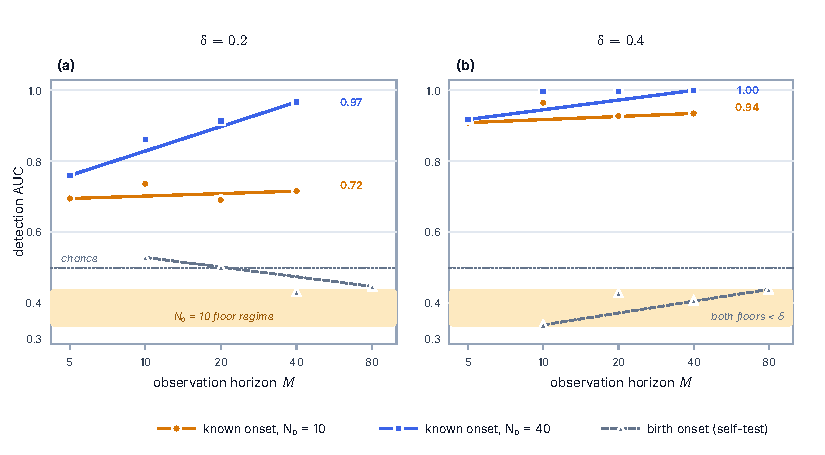
\includegraphics[width=\columnwidth]{anthro/fig2_onset.pdf}
\Description{Two panels, one per deception footprint, plotting detection
AUC against the observation horizon on a log scale. Two solid curves for a
known-onset attacker with 10 and 40 memorized reference turns rise to
plateaus of different heights, one pair saturating near one and the other
pair stalling in the 0.7 to 0.97 range. A dashed birth-onset curve
oscillates slightly below the chance line at every horizon.}
\caption{E5: onset regimes on constructed planes (all frozen values).
Detection AUC of the two-sample statistic vs.\ fresh-sample horizon $M$;
one panel per footprint $\delta$. Solid curves memorize a reference batch
($N_0=10$, $N_0=40$); the dashed curve is the birth-onset self-test
($N_0=0$), whose registered ``flat at chance'' prediction failed: it reads
$0.431$--$0.529$ at $\delta=0.2$ (two of the four readings below chance)
and $0.339$--$0.439$ at $\delta=0.4$,
up to $0.16$ \emph{below} chance (a small-sample asymmetry of the
studentized statistic: with $N_0=0$ the reference stream doubles as the
first half of the $M$-sample draw, so the lattice of the score's null
distribution sits a half step below chance at short $M$, and the
plug-in variance from the same path is conservative by design of the
two-sample plug-in). Plateaus: $(10,0.2)$ flat at
$0.69$--$0.74$, $19$--$24$ points above chance; $(40,0.2)$ rising to
$0.97$; $(10,0.4)$ non-monotone $0.91$--$0.97$; $(40,0.4)$ $0.92\to1.000$.
The corrected boundary $\Delta_{\beta_d}=1.84\rho_0$ orders the extremes;
the shaded band marks the $N_0=10$ reference-width regime.}
\label{fig:onset}
\end{figure}

\paragraph{The post hoc ordinal reading (exploratory)}
Figure~\ref{fig:onset} plots the frozen cells, and Table~\ref{tab:widths}
reads them against the \emph{corrected} boundaries---labeled post hoc
because neither the corrected boundary nor the ordinal comparison appears
in the registration: the registered floors are
$\rho_0=0.284$ and $0.142$ at $N_0=10$ and $40$ ($z=1.96$, $p=0.30$; the
earlier draft printed $0.283/0.141$), the certified boundaries are
$\Delta_{\beta_d}=0.522$ and $0.261$, and the non-adaptive width
$w_{\mathrm{na}}=0.774/0.387$ bounds what a threshold fixed independently
of the honest rate can reach. The reading is qualitative at the middle
cells: $\Delta_{\beta_d}$ orders the extremes (the below-width cell is
capped and lowest; the certified cell alone reaches $1.000$, with
$M^{*}\approx30$ and AUC saturation preceding the certified-power
threshold because AUC pools all thresholds), but the two middle cells'
plateaus overlap ($0.76\to0.97$ rising vs.\ $0.91$--$0.97$ non-monotone)
and admit no strict ordinal claim. The adaptive minimax boundary between
the regimes remains open (Section~\ref{sec:discussion}). The instrument
any reviewer can rerun did its job: it falsified the registered
prediction at three cells, falsified the earlier draft's statement of
this theorem at the middle cells, and now anchors a corrected statement
whose certified horizon matches the only cell that saturates.

\begin{table}[t]\centering\footnotesize
\begin{tabular}{ccccccl}
\toprule
$N_0$ & $\delta$ & $\rho_0$ & $\Delta_{\beta_d}$ & $w_{\mathrm{na}}$ &
regime (restated Thm.~\ref{thm:onset}) & observed AUC (all $M$) \\
\midrule
10 & 0.2 & 0.284 & 0.522 & 0.774 & below width: cap $L\rho_0$ & $0.69$--$0.74$, flat \\
40 & 0.2 & 0.142 & 0.261 & 0.387 & middle: uncertified power $\forall M$ & $0.76\to0.97$ \\
10 & 0.4 & 0.284 & 0.522 & 0.774 & middle: uncertified power $\forall M$ & $0.91$--$0.97$, non-monotone \\
40 & 0.4 & 0.142 & 0.261 & 0.387 & certified: $M^{*}\!\approx\!30$ & $0.92\to1.000$ \\
\bottomrule
\end{tabular}
\caption{The registered E5 prediction versus the corrected boundaries
(exploratory, post hoc; $\beta_d=0.05$ two-sided; $p=0.30$;
$\rho_0=z_{1-\beta_d/2}\sqrt{p(1-p)/N_0}=0.284/0.142$;
$\Delta_{\beta_d}=(z_{1-\beta_d/2}+z_{1-\beta_d})\sigma_0=1.84\rho_0=0.522/0.261$;
non-adaptive width $w_{\mathrm{na}}=\sqrt{2\ln(1/\beta_d)/N_0}=0.774/0.387$;
observed values frozen, all four $M$ points per cell). The registered
prediction (``advantage $\to1$ above the floor; flat at chance'') failed
at three cells (Section~\ref{sec:e5}); the corrected trichotomy orders the
extremes and leaves the two middle cells overlapping plateaus below
certified power (limiting TPR $0.79$ normal; the one-sided exact binomial
UMP has power $0.850$ at $(10,0.4)$ and $0.807$ at $(40,0.2)$).}
\label{tab:widths}
\end{table}
